Chapter% Itt kezdődik a dolgozat lényegi része, úgy értve, hogy a saját munka bemutatása.
% Jellemzően ebben szerepelni szoktak blokkdiagramok, a program struktúrájával foglalkozó leírások.
% Ehhez célszerű UML ábrákat (például osztály- és szekvenciadiagramokat) használni.

% Amennyiben a dolgozat inkább kutatás jellegű, úgy itt lehet konkretizálni a kutatási módszertant, a kutatás tervezett lépéseit, az indoklást, hogy mit, miért és miért pont úgy érdemes csinálni, ahogyan az a későbbiekben majd részletezésre kerül.

% Ebben a fejezetben az implementáció nem kell, hogy túl nagy szerepet kapjon.
% Ez még csak a tervezési fázis.
% (Nyilván ha olyan a téma, hogy magának az implementációnak a módjával foglalkozik, adott formális nyelvet mutat be, úgy a kódpéldákat már innen sem lehet kihagyni.)

% \Section{Táblázatok}

% Táblázatokhoz a \texttt{table} környezetet ajánlott használni.
% Erre egy minta \aref{tab:minta}. táblázat.
% A hivatkozáshoz az egyedi \texttt{label} értéke konvenció szerint \texttt{tab:} prefixszel kezdődik.

% \begin{table}[h]
% \centering
% \caption{Minta táblázat. A táblázat felirata a táblázat felett kell legyen!}
% \label{tab:minta}
% \begin{tabular}{l|c|c|}
% a & b & c \\
% \hline
% 1 & 2 & 3 \\
% 4 & 5 & 6 \\
% \hline
% \end{tabular}
% \end{table}

% \Section{Ábrák}

% Ábrákat a \texttt{figure} környezettel lehet használni.
% A használatára egy példa \aref{fig:cimer}. ábrán látható.
% Az \texttt{includegraphics} parancsba 
% Az ábrák felirata az ábra alatt kell legyen.
% Az ábrák hivatkozásához használt nevet konvenció szerint \texttt{fig:}-el célszerű kezdeni.

% \begin{figure}[h]
% \centering
% 
\includegraphics[scale=0.3]{images/me_logo.png}
% \caption{A Miskolci Egyetem címere.}
% \label{fig:cimer}
% \end{figure}

% \Section{További környezetek}

% A matematikai témájú dolgozatokban szükség lehet tételek és bizonyításaik megadására.
% Ehhez szintén vannak készen elérhető környezetek.

% \begin{definition}
% Ez egy definíció
% \end{definition}

% \begin{lemma}
% Ez egy lemma
% \end{lemma}

% \begin{theorem}
% Ez egy tétel
% \end{theorem}

% \begin{proof}
% Ez egy bizonyítás
% \end{proof}

% \begin{corollary}
% Ez egy tétel
% \end{corollary}

% \begin{remark}
% Ez egy megjegyzés
% \end{remark}

% \begin{example}
% Ez egy példa
% \end{example}

\Chapter{Tervezés}

\Section{Kinézet}
A kinézetet játékos, egyszerű és átláthatóra szeretném csinálni.
Mindenhol játékos ikonokat és színvilágot szeretnék használni, az oldal ikonja az alábbi lenne:

\begin{figure}[h]
    \centering
    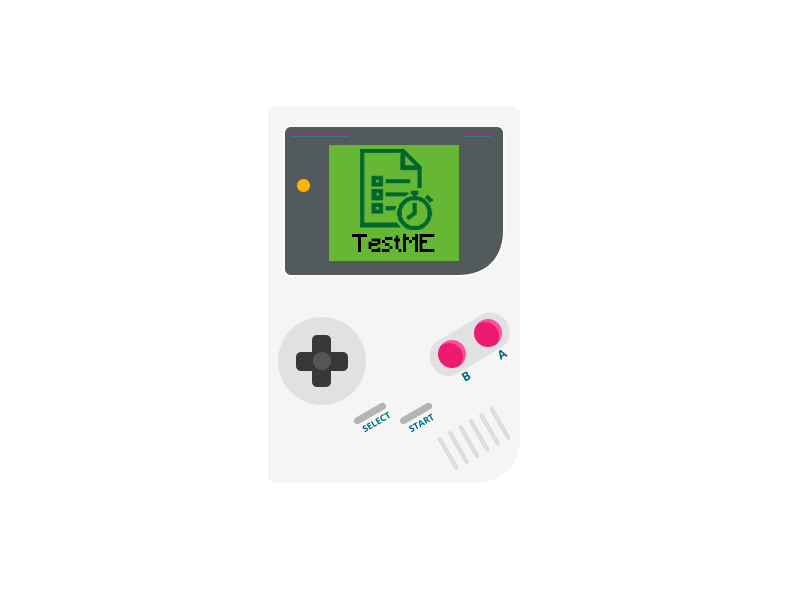
\includegraphics[height=5cm]{images/gameboy.png}
\end{figure}


Minden grafikus elem szeretném hogy egységes legyen így törekedtem arra hogy hasonló stílusú legyen minden. Az egyéb funkciókhoz vagy oldalakhoz társított ikonok, amelyek az oldalt még játékosabbá tennék pedig az alábbiak lennének:

\begin{figure}[h]
    \begin{subfigure}{.1\textwidth}
        \centering
        
\includegraphics[width=.8\linewidth]{images/icons/003-swords.png}
    \end{subfigure}
    \begin{subfigure}{.1\textwidth}
        \centering
        
\includegraphics[width=.8\linewidth]{images/icons/005-fists.png}
    \end{subfigure}
    \begin{subfigure}{.1\textwidth}
        \centering
        
\includegraphics[width=.8\linewidth]{images/icons/006-gamer.png}
    \end{subfigure}
    \begin{subfigure}{.1\textwidth}
        \centering
        
\includegraphics[width=.8\linewidth]{images/icons/007-gamer.png}
    \end{subfigure}
    \begin{subfigure}{.1\textwidth}
        \centering
        
\includegraphics[width=.8\linewidth]{images/icons/014-computer.png}
    \end{subfigure}
    \begin{subfigure}{.1\textwidth}
        \centering
        
\includegraphics[width=.8\linewidth]{images/icons/028-trophy.png}
    \end{subfigure}
    \begin{subfigure}{.1\textwidth}
        \centering
        
\includegraphics[width=.8\linewidth]{images/icons/030-flag.png}
    \end{subfigure}
    \begin{subfigure}{.1\textwidth}
        \centering
        
\includegraphics[width=.8\linewidth]{images/icons/052-rank.png}
    \end{subfigure}
    \begin{subfigure}{.1\textwidth}
        \centering
        
\includegraphics[width=.8\linewidth]{images/icons/053-sword.png}
    \end{subfigure}
    \begin{subfigure}{.1\textwidth}
        \centering
        
\includegraphics[width=.8\linewidth]{images/icons/054-sword.png}
    \end{subfigure}
    \begin{subfigure}{.1\textwidth}
        \centering
        
\includegraphics[width=.8\linewidth]{images/icons/057-computer.png}
    \end{subfigure}
    \begin{subfigure}{.1\textwidth}
        \centering
        
\includegraphics[width=.8\linewidth]{images/icons/058-potion.png}
    \end{subfigure}
\end{figure}


Valamint Bootstrap-et szeretnék használni ami egy olyan keretrendszer, amely segít a weboldalak gyorsabb és könnyebb megtervezésében. HTML és CSS alapú tervezősablonokat tartalmaz a tipográfiához, űrlapokat, gombokat, táblázatokat, navigációt, modelleket stb. Ez segítene abban hogy az oldalon egységet kinézetet hozhassak létre valamit a Bootstrap CSS-je alkalmazkodik a telefonokhoz, táblagépekhez és asztali számítógépekhez is.

Ehhez egy ingyenes Bootstrap témát választottam ami szerintem menne a weboldal témájához, ezt a témát Litera-nak\cite{litera} hívják.

\Section{Funkciók}

\begin{itemize}
    \item {Bejelentkezés/Regisztráció}
          \begin{addmargin}[\parindent]{0pt}
              Az weboldal megnyitásakor a felhasználónak be kell jelentkeznie vagy egy helyes e-mail címmel és egy kellően biztonságos jelszóval, regisztrálni kell ha használni szeretné az oldalt.
          \end{addmargin}
    \item {Tesztkészítés}
          \begin{addmargin}[\parindent]{0pt}
              Kahoot!-hoz hasonló teszt készítési felületet szeretnék létrehozni ahol az elkészített teszteket hozzá lehet rendelni diákokhoz és ezután kitölthetik azokat.
          \end{addmargin}
    \item {Pontgyűjtés}
          \begin{addmargin}[\parindent]{0pt}
              Minden regisztrált felhasználó rendelkezik majd egy szinttel és egy bizonyos pontszámmal, amelyet a tesztek kitöltésével szerezhetnek.
          \end{addmargin}
    \item {Ranglista}
          \begin{addmargin}[\parindent]{0pt}
              Ranglista a teszt teljes kitöltését követően alakul ki a legtöbbet szerzett pontok alapján.
          \end{addmargin}
    \item {Felhasználói szerepkörök kezelése}
          \begin{addmargin}[\parindent]{0pt}
              Különböző szerepkörök lennének amik azzal bírnának hogy egy tanár jogosultságú felhasználó hozhat létre tesztet és hozzá rendelheti diákokhoz. A diák pedig csak kitölthetné azt.
          \end{addmargin}
    \item {Tesztek diákhoz rendelése}
          \begin{addmargin}[\parindent]{0pt}
              Teszt létrehozása során email cím vagy valamilyen más egyedi azonosító segítségével hozzá lehetne rendelni diákokhoz a tesztet és így értesülnének róla hogy ki kell tölteniük.
          \end{addmargin}
    \item {Összes hozzárendelt teszt megtekintése}
          \begin{addmargin}[\parindent]{0pt}
              Diákként meg lehet nézni az összes olyan tesztet amit valaki hozzá rendelt a profilhoz. És ezzel együtt a régiek eredményét is, hogy az hogy sikerült mindenkinek.
          \end{addmargin}
\end{itemize}

\subsection{Elérési módjuk}

Az oldalon lévő minden funkciót csak regisztráció vagy bejelentkezés után lehet használni. Ez azért fontos hiszen csak így lehet a felhasználónak tesztet küldeni és kitöltés után csak így lehet hozzáadni a profiljához a pontokat és megjeleníteni a nevét a ranglistán.

\vspace{5mm}

\noindent Regisztrálni lehet majd tanár és diákként. Ez a kettő azért van szétválasztva hogy a diákok jogosultsági körét korlátozni lehessen, például hogy egy diák ne írhasson egy tesztet és rendelje hozzá a tanárjához. Tehát ez a két funkció csak tanárok számára elérhető.

\subsection{Használati eset}

Itt látható egy kezdetleges használati eset-modell (use case diagram) ebben benne van a felhasználók információs igényeinek elemzése, funkcionális követelmények elemzése és a modell tartalmazza a rendszerrel szemben támasztott felhasználói követelményeket.
Látszik hogy kik (esetünkben tanár és diák) és mire akarják használni a rendszert.

\begin{figure}[h]
    \centering
    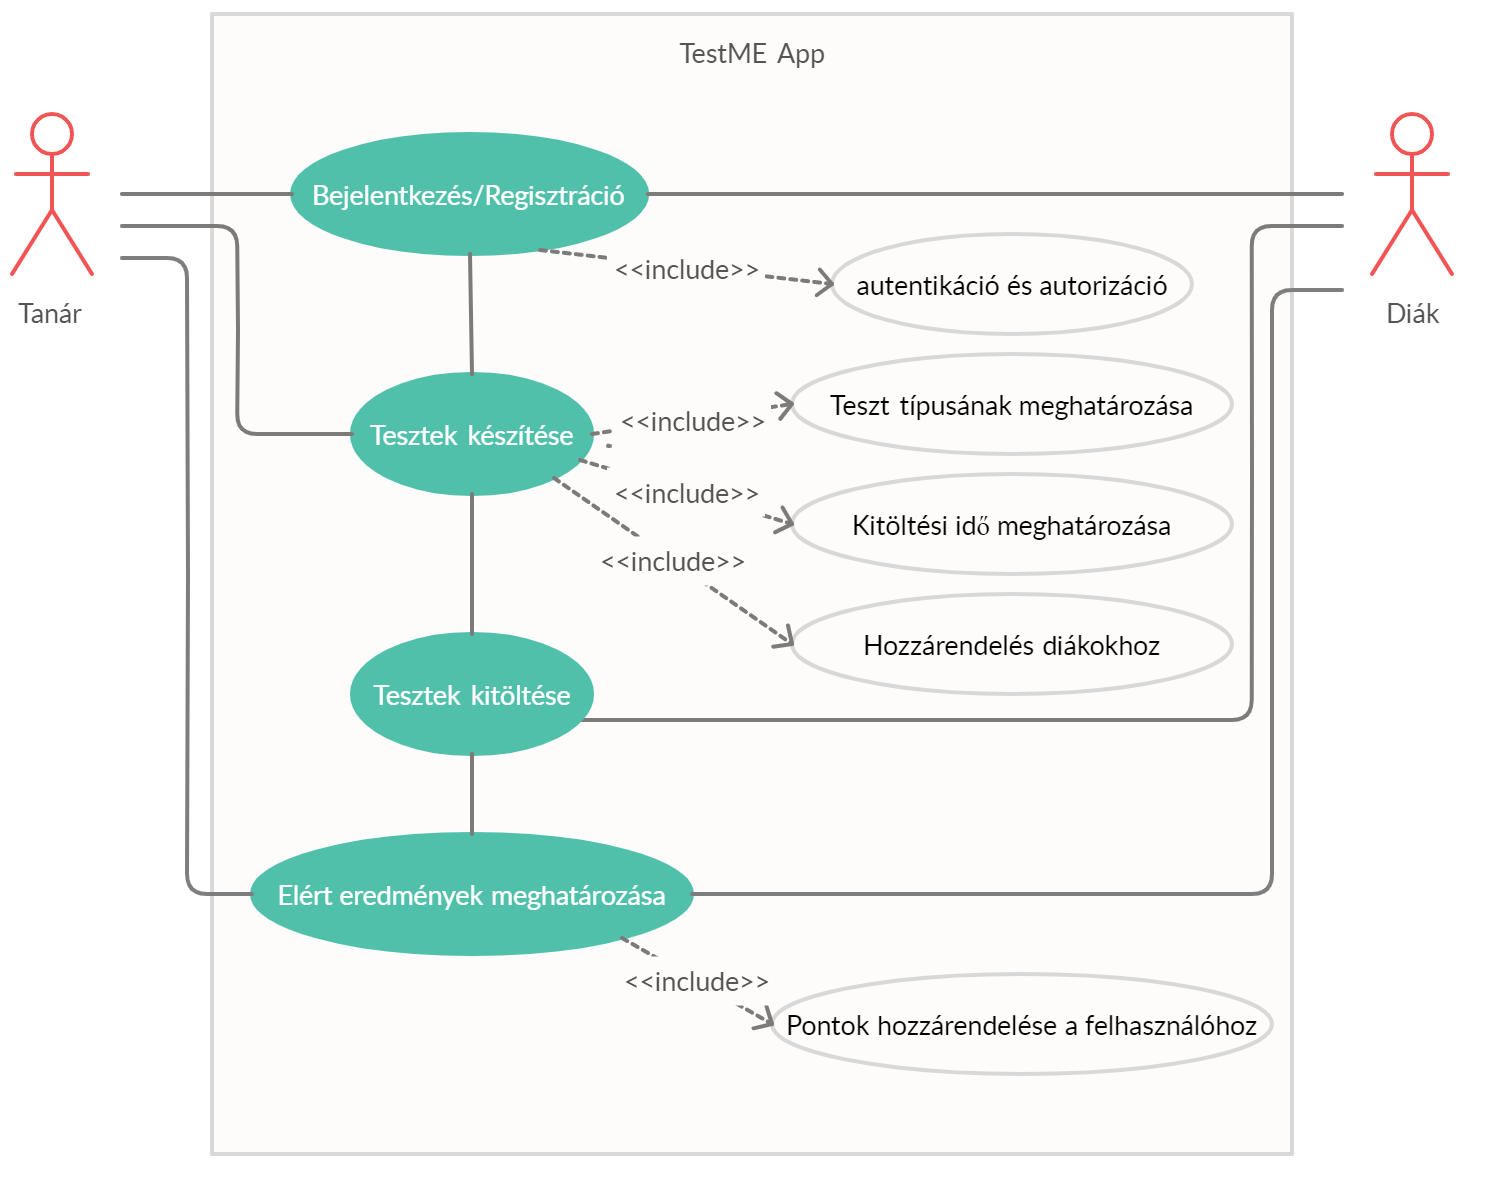
\includegraphics[width=12cm]{images/use_case.png}
    \caption{Használati eset-modell}
\end{figure}
